% =============================================================================
%  main.tex -- Journal of Supercomputing (Springer) submission, Embedded
%  Systems section.
%
%  Uses the Springer Nature "sn-jnl" class. Before compiling:
%    1. Download the current Springer Nature LaTeX template package from
%       https://www.springernature.com/gp/authors/campaigns/latex-author-support
%       and place sn-jnl.cls (and sn-mathphys-num.bst, if you switch to
%       BibTeX) next to this file.
%    2. Double-check the documentclass option below (sn-mathphys, Numbered)
%       against the *current* Journal of Supercomputing author guidelines --
%       Springer occasionally changes the required reference style per
%       journal.
%    3. This file compiles cleanly (verified with tectonic + a GitHub
%       mirror of sn-jnl.cls: godkingjay/springer-nature-latex-template).
%       Before submission, re-verify against the *official* sn-jnl.cls
%       from Springer's own author-support download (mirrors can drift
%       from the version a specific journal expects).
%    4. A few bibliography entries are flagged "VERIFY" below: the exact
%       volume/page/DOI could not be independently confirmed while writing
%       this file offline. Please confirm them against the publisher
%       record before submission.
% =============================================================================
\documentclass[pdflatex,sn-mathphys,Numbered]{sn-jnl}

\usepackage{graphicx}
\usepackage{multirow}
\usepackage{amsmath,amssymb,amsfonts}
\usepackage{manyfoot}
\usepackage{booktabs}
\usepackage{algorithm}
\usepackage{algpseudocode}
\usepackage{xcolor}
\usepackage{tikz}
\usetikzlibrary{shapes.geometric,positioning,arrows.meta,fit,backgrounds}
\usepackage{hyperref}

\raggedbottom

\begin{document}

\title[Surface-Code QEC on a 28-Qubit FPGA Statevector Simulator]{Hardware-in-the-Loop Verification of Distance-3 Surface-Code Quantum Memory on a 28-Qubit HBM-Accelerated FPGA Statevector Simulator}

\author*[1]{\fnm{Nasir} \sur{Ali}}\email{nasirali2607@gmail.com}

\affil*[1]{\orgdiv{Embedded Systems Division}, \orgname{Centre for Development of Advanced Computing (C-DAC)}, \orgaddress{\city{Noida}, \postcode{201307}, \state{Uttar Pradesh}, \country{India}}}

\abstract{Surface codes are the leading practical route to fault-tolerant quantum computation, but validating the classical control and decoding stack that a surface-code memory needs -- repeated syndrome extraction, ancilla reset, and syndrome-history decoding -- ordinarily requires either scarce physical qubits or a Clifford-only stabilizer simulator that discards the full quantum state. This paper reports an implementation of a distance-3 rotated surface code (9 data and 8 ancilla qubits, of 28 addressable) on an HBM-resident, complex128 FPGA statevector accelerator (AMD/Xilinx Alveo U55C), and shows how to run a genuine multi-round fault-tolerant memory experiment on hardware that -- like many first-generation statevector accelerators -- exposes no native mid-circuit measurement-and-branch primitive. Every entangling operation (synthetic error injection, ancilla reset, and the measure-$Z$/measure-$X$ syndrome-extraction circuits) executes as a real unitary circuit on the FPGA kernel each round; only the unavoidable measurement collapse and the classical minimum-weight-perfect-matching (MWPM) decoding run on the host, mirroring the classical/quantum division of labour the theory itself prescribes. The full stabilizer set, logical-operator pair, and decoding graph were derived from first principles and independently verified against \texttt{qiskit.quantum\_info} (93 algebraic and decoding-logic assertions, all passing); every hardware trial additionally cross-checks the FPGA-computed statevector's logical readout against an independently tracked classical Pauli frame, catching a real decoding-graph connectivity bug during development. Across a physical-error-rate sweep on real hardware (150 trials, 600 FPGA-executed syndrome rounds, zero cross-validation discrepancies), the decoded logical error rate is consistent with zero at $p=1\%$ and rises sharply above it, in qualitative agreement with the accuracy threshold reported by Dennis, Kitaev, Landahl and Preskill. We discuss the engineering trade-offs of the host-mediated protocol, a decoding-graph construction pitfall we found and fixed, and the throughput gap between this exact-statevector validation approach and dedicated real-time surface-code decoder pipelines.}

\keywords{quantum error correction, surface codes, FPGA acceleration, statevector simulation, HBM, minimum-weight perfect matching, syndrome extraction, embedded quantum control systems}

\maketitle

% =============================================================================
\section{Introduction}\label{sec:intro}
% =============================================================================

Surface codes~\cite{kitaev2003,bravyikitaev1998,dennis2002,fowler2012} are, by consensus, the most experimentally mature route to fault-tolerant quantum computation: their stabilizer generators act only on geometrically local groups of qubits, they tolerate physical error rates on the order of $10^{-2}$--$10^{-3}$, and superconducting-qubit demonstrations have now shown logical error suppression that scales as the code distance grows~\cite{acharya2023}. All of these demonstrations, however, depend on a substantial classical control and decoding stack: syndrome bits must be extracted every cycle, ancillas reset, a running syndrome history assembled into a space-time detector graph, and a minimum-weight matching (or equivalent) decoder must return a correction fast enough to keep pace with the physical cycle time. Developing and validating that classical stack does not, in principle, require physical qubits at all -- but it does require a simulation substrate that (a) reproduces the true quantum state closely enough to serve as ground truth, and (b) is realised on hardware whose execution model forces the same architectural choices a real control system must make.

Two families of tools sit at the extremes of this design space. Stabilizer-only simulators such as Stim~\cite{gidney2021stim} are extremely fast because they never materialise a $2^{n}$-dimensional state vector, but that speed comes from restricting the simulated circuit to the Clifford group -- adequate for most surface-code memory studies, but not for future work that couples QEC circuits to non-Clifford resource states, coherent errors, or leakage. At the other extreme, full statevector simulation retains the exact quantum state at the cost of exponential memory, which is why FPGA- and GPU-accelerated statevector engines with high-bandwidth memory (HBM) have become an active area of embedded/accelerator systems research, including our own prior work on FPGA-resident statevector, density-matrix and matrix-product-state engines for the same Alveo U55C hardware family~\cite{ali_rtl_statevector,ali_30qubit_sim,ali_mps_engine}. What has not, to our knowledge, been previously reported is a full multi-round surface-code syndrome-extraction-and-decode loop executed on such a statevector accelerator, with an explicit protocol for the case -- common to many first-generation FPGA/GPU statevector kernels, including the one used here and in a companion real-time-decoder study~\cite{ali_shor_steane_qec} -- where the accelerator itself offers no native mid-circuit measurement-and-classically-conditioned-branch instruction.

This absence is not a minor implementation detail. A textbook description of repeated stabilizer measurement (e.g. Fowler et al.'s measure-$Z$/measure-$X$ circuits~\cite{fowler2012}) implicitly assumes the device can measure an ancilla, branch on the outcome, reset it, and continue -- all within one coherent circuit. Many statevector kernels instead expose only (i) fully unitary gate sequences and (ii) an end-of-circuit, Born-rule sample of the final state; a hardware \texttt{reset} instruction, where present, typically performs a deterministic projection rather than returning a classical outcome a subsequent gate could condition on. Section~\ref{sec:protocol} shows how to build a faithful, verifiable multi-round QEC memory experiment on top of exactly these two primitives, by dispatching one purely unitary circuit per syndrome round to the accelerator and performing only the physically unavoidable measurement collapse and the classical decoding on the host -- which is, in fact, precisely the division of labour the surface-code fault-tolerance literature itself prescribes for the quantum device versus its classical controller~\cite{dennis2002}.

\subsection{Contributions}
\begin{enumerate}
\item A distance-3 rotated surface code (9 data qubits, 8 ancilla qubits, 17 of 28 addressable qubits) whose stabilizer generators, logical operator pair and decoding-graph boundary connectivity are derived from first principles -- not copied from a published figure -- and independently verified against an exact linear-algebra reference (\texttt{qiskit.quantum\_info}), reported as a reusable derivation method in Section~\ref{sec:code}.
\item A host/FPGA co-execution protocol for multi-round syndrome extraction on an accelerator with no native mid-circuit classical feedback (Section~\ref{sec:protocol}), in which every entangling and error-injection operation still executes on the FPGA kernel and only measurement collapse and decoding run on the host.
\item A synthetic-syndrome-data generator implementing the Dennis--Kitaev--Landahl--Preskill error model~\cite{dennis2002}, in which qubit bit-flip errors, qubit phase-flip errors and syndrome-readout errors all occur at the same rate $p$, giving controlled, repeatable QEC benchmarking without physical qubits.
\item A from-scratch space-time minimum-weight-matching decoder, exact for the small instances this code produces, together with a documented decoding-graph construction pitfall we found and fixed during development (Section~\ref{sec:decoder}) -- restricting boundary connectivity to weight-2 "boundary" stabilizers only, which under-connects the graph and lets certain weight-1 physical errors decode to a logical error, violating the distance-3 guarantee.
\item An end-to-end hardware/software cross-validation methodology in which every trial's FPGA-computed statevector logical readout is checked against an independently tracked classical Pauli frame, giving a built-in correctness oracle for the whole pipeline (Section~\ref{sec:results}).
\item Experimental results on real Alveo U55C hardware across a physical-error-rate sweep (Section~\ref{sec:results}), reproducing the qualitative threshold behaviour reported in~\cite{dennis2002}.
\end{enumerate}

The remainder of the paper is organised as follows. Section~\ref{sec:related} surveys related work in surface-code theory, decoding, and FPGA/GPU-accelerated quantum simulation. Section~\ref{sec:background} summarises the surface-code formalism and the FPGA statevector accelerator's architecture and execution model. Section~\ref{sec:code} derives and verifies the distance-3 code instance used throughout. Section~\ref{sec:protocol} presents the host/FPGA co-execution protocol and synthetic-syndrome-data generator. Section~\ref{sec:decoder} describes the space-time decoding graph and the matching decoder. Section~\ref{sec:setup} details the experimental setup, and Section~\ref{sec:results} reports and discusses the results. Section~\ref{sec:conclusion} concludes and outlines future work.

% =============================================================================
\section{Related work}\label{sec:related}
% =============================================================================

\textbf{Surface-code theory.} Kitaev's toric code~\cite{kitaev2003} and its planar (boundary-truncated) variants~\cite{bravyikitaev1998} underlie the modern surface code. Dennis, Kitaev, Landahl and Preskill~\cite{dennis2002} formalised the accuracy-threshold analysis this paper's error model follows, including the observation that qubit bit-flip errors, qubit phase-flip errors and syndrome-measurement errors can be treated at a common probability $p$ for threshold estimation purposes. Fowler, Mariantoni, Martinis and Cleland~\cite{fowler2012} gave the concrete measure-$Z$/measure-$X$ ancilla circuits this paper implements verbatim, and estimated physical-qubit overheads for large-scale factoring circuits. Tomita and Svore~\cite{tomita2014} studied small-distance rotated surface codes under realistic circuit-level noise and identified the hook-error-optimal CNOT scheduling that Section~\ref{sec:code} explicitly does \emph{not} implement (a scoped simplification discussed in Section~\ref{sec:discussion}). Versluis et al.~\cite{versluis2017} describe a scalable control architecture for a distance-3 rotated surface code on superconducting hardware; the lattice used here was derived independently from first principles (Section~\ref{sec:code}) rather than reproduced from that or any other single reference. Google Quantum AI's 2023 demonstration~\cite{acharya2023} showed logical error suppression with increasing code distance on real superconducting hardware, the experimental benchmark against which classical-control simulation work such as this paper is ultimately positioned. IBM's heavy-hexagon subsystem-code work~\cite{chamberland2020} is a further example of hardware-aware code design trading stabilizer weight for connectivity constraints, a consideration directly relevant to any future port of this methodology to a different accelerator topology.

\textbf{Decoding.} Minimum-weight perfect matching traces to Edmonds' blossom algorithm~\cite{edmonds1965}; Higgott's PyMatching~\cite{higgott2022} is the de facto standard practical implementation for surface-code decoding graphs at scale, and Delfosse and Nickerson's Union-Find decoder~\cite{delfosse2021} targets near-linear-time decoding for real-time use. This paper implements its own small, exact (brute-force, boundary-augmented) MWPM solver rather than depending on an external decoding library, since the distance-3 instance studied here produces at most a handful of simultaneous detection events per trial (Section~\ref{sec:decoder}); adopting PyMatching or a Union-Find decoder is identified as necessary future work for larger code distances (Section~\ref{sec:discussion}).

\textbf{Classical simulation of QEC circuits.} Stim~\cite{gidney2021stim} simulates stabilizer circuits at very high throughput but is restricted to the Clifford group, which this paper's synthetic-error-injection circuits happen to respect but which a full statevector engine is not restricted to; the value of the present approach is precisely that it does not rely on that restriction, at the cost of the exponential memory a statevector representation requires.

\textbf{FPGA/GPU-accelerated quantum simulation.} This work reuses the HBM-resident, complex128 statevector kernel architecture described in a companion submission~\cite{ali_rtl_statevector}, part of a broader indigenous FPGA quantum-simulation effort at C-DAC that also includes a 30-qubit statevector engine~\cite{ali_30qubit_sim}, an FPGA matrix-product-state engine~\cite{ali_mps_engine}, and a dedicated real-time LUT/Union-Find/MWPM decoder pipeline targeting sub-microsecond syndrome-to-correction latency on the same Alveo U55C hardware family~\cite{ali_shor_steane_qec}. That decoder pipeline and the present paper are complementary rather than overlapping: the former targets decoding \emph{latency} on physically streamed syndrome data for Shor and Steane codes, whereas this paper targets \emph{algorithmic correctness validation} of a full surface-code memory protocol against an exact simulated quantum state, at wall-clock timescales orders of magnitude slower than a real decoding cycle (Section~\ref{sec:discussion}). NVIDIA's CUDA-Q / CUDA-QX (\texttt{cudaq-qec}) toolkit represents a GPU-accelerated approach to the same broader problem space and is noted here as related, complementary tooling rather than a baseline this paper benchmarks against.

To the best of our knowledge, no prior work reports a full multi-round surface-code syndrome-extraction-and-decode loop, cross-validated against an exact statevector, on FPGA-accelerated hardware whose execution model lacks native mid-circuit classical feedback, together with an explicit, reusable protocol for that constraint. That is the gap this paper addresses.

% =============================================================================
\section{Background}\label{sec:background}
% =============================================================================

\subsection{Rotated surface codes and the accuracy threshold}\label{sec:background-surface}

A distance-$d$ rotated surface code encodes one logical qubit into $2d^{2}-1$ physical qubits: $d^{2}$ data qubits carrying the code's Pauli-$X$/$Z$ degrees of freedom, and $d^{2}-1$ ancilla qubits, each measuring one stabilizer generator. Stabilizers come in two flavours -- $X$-type, $\hat X_{a}\hat X_{b}\hat X_{c}\hat X_{d}$ (weight 4 in the bulk, weight 2 at one pair of boundaries), and $Z$-type, $\hat Z_{a}\hat Z_{b}\hat Z_{c}\hat Z_{d}$ (weight 4 in the bulk, weight 2 at the other pair of boundaries) -- chosen so that every $X$-type and every $Z$-type generator commutes (even qubit-support overlap), while the code's two logical operators $\bar X$, $\bar Z$ each commute with every stabilizer and anticommute with each other. Physical Pauli errors that anticommute with a stabilizer flip its measured eigenvalue (a \emph{detection event}); a classical decoder infers a correction from the pattern of detection events, typically by minimum-weight matching on a graph whose edges represent the physical errors most likely to explain a given syndrome~\cite{dennis2002,fowler2012}.

Dennis, Kitaev, Landahl and Preskill~\cite{dennis2002} showed that, under a model in which qubit bit-flip errors, qubit phase-flip errors and syndrome-measurement errors all occur independently with the same probability $p$ per qubit per round, there is an accuracy threshold $p_{c}$ (estimated at $p_c \gtrsim 1.14\%$ for their optimal-recovery bound) below which increasing the code distance suppresses the logical error rate arbitrarily; above threshold, larger codes perform worse. This paper's error model and its "quantum memory" experiment design (encode, apply repeated noisy syndrome rounds, decode once, and check whether the logical value survived) follow that construction directly (Section~\ref{sec:protocol}).

\subsection{The FPGA statevector accelerator}\label{sec:background-fpga}

The target platform is an AMD/Xilinx Alveo U55C accelerator card hosting a custom HLS kernel (\texttt{quantum\_fpga\_kernel\_complex128}, compiled from a C++ HLS source via Vitis) that maintains a $2^{n}$-amplitude complex128 statevector across two HBM-resident arrays -- one for the real part, one for the imaginary part -- each striped across 8 HBM pseudo-channels (256\,MB each, 2\,GB per array). With $2^{n}$ amplitudes $\times$ 8 bytes (double) $=2$\,GB exactly at $n=28$, the kernel's HBM allocation caps addressable circuits at $\text{MAX\_QUBITS\_FPGA}=28$ without widening the per-array HBM range. A third, smaller HBM-resident buffer carries the gate stream: each gate is encoded as an 8-word record (opcode, up to three qubit indices, and up to three packed single-precision parameters), and up to 512 gates are dispatched per kernel launch.

The kernel natively executes 19 opcodes (identity, the seven single-qubit Clifford/Pauli gates $H,X,Y,Z,S,S^\dagger,\sqrt X, \sqrt X^\dagger$, $T/T^\dagger$, the parametrised rotations $R_x,R_y,R_z,P,U_2,U_3$, and the two-qubit entanglers CX and CZ). A host-side lowering pass decomposes every other supported gate (SWAP, controlled-$Y$/$H$/$R_x$/$R_y$/$R_z$/$\sqrt X$, DCX, iSWAP, ECR, $R_{xx}/R_{yy}/R_{zz}$, Toffoli, and general multi-controlled-$X$) into this native basis using standard circuit identities before dispatch, so that every circuit the host driver accepts ultimately reduces to single-qubit rotations plus CX/CZ on the kernel itself.

Two properties of this execution model shape the protocol design in Section~\ref{sec:protocol}. First, a \texttt{reset} instruction deterministically projects a qubit onto $\lvert 0\rangle$ (zeroing the amplitudes with that qubit set to $1$ and renormalising) rather than returning a classical outcome; second, \texttt{measure} instructions are resolved only at the end of a circuit, by Born-rule sampling of the final statevector, and the driver returns the exact pre-sampling statevector alongside the sampled bitstrings. There is no instruction that measures a qubit \emph{mid-circuit} and conditions a subsequent gate on the outcome. This is a common characteristic of first-generation FPGA/GPU statevector kernels (including our own prior work~\cite{ali_rtl_statevector,ali_30qubit_sim}), and is the constraint Section~\ref{sec:protocol} is designed around, rather than a limitation specific to surface-code circuits.

The host driver exposes this kernel through a Qiskit-compatible Python API over AMD's Xilinx Runtime (XRT); circuits are supplied as gate tuples, executed via one or more kernel launches per circuit, and returned as the exact final statevector together with Born-rule-sampled measurement outcomes.

% =============================================================================
\section{Distance-3 rotated surface code: derivation and verification}\label{sec:code}
% =============================================================================

\subsection{Lattice derivation}

Rather than reproduce a published lattice diagram, the code instance used throughout was derived directly from the stabilizer-commutation requirement, as a reusable method applicable to any code distance within a target qubit budget. Nine data qubits $q_{0},\dots,q_{8}$ are placed on a $3\times3$ grid, indexed $q_{3y+x}$ for $(x,y)\in\{0,1,2\}^{2}$. Candidate ancilla positions are placed at every half-integer coordinate $(x+\tfrac12,y+\tfrac12)$ for $x,y\in\{-1,0,1,2\}$ (one ring of padding around the data grid), and a candidate is discarded if it neighbours fewer than two data qubits (the four lattice corners). Each surviving candidate is coloured by the parity of $x+y$: one colour becomes an $X$-type ancilla, the other $Z$-type. At each of the four physical edges, exactly one of the two colour-alternating boundary candidates is kept, chosen so that $X$-type ancillas are truncated to weight 2 on the top/bottom edges and $Z$-type ancillas on the left/right edges. This yields the eight stabilizer generators in Table~\ref{tab:stabilizers} and the qubit layout in Figure~\ref{fig:lattice}: four $X$-type (detecting $Z$ errors) and four $Z$-type (detecting $X$ errors), for $9+8=17$ of the 28 available qubits.

\begin{table}[t]
\centering
\caption{Stabilizer generators and logical operators of the distance-3 rotated surface code used in this work. Ancilla qubit indices: $\mathrm{XS}_{0\text{--}3}\mapsto q_{9\text{--}12}$, $\mathrm{ZS}_{0\text{--}3}\mapsto q_{13\text{--}16}$.}
\label{tab:stabilizers}
\begin{tabular}{@{}llll@{}}
\toprule
Generator & Support & Type & Boundary \\
\midrule
$\mathrm{XS}_0$ & $q_0,q_1$ & weight 2 & top \\
$\mathrm{XS}_1$ & $q_1,q_2,q_4,q_5$ & weight 4 & interior \\
$\mathrm{XS}_2$ & $q_3,q_4,q_6,q_7$ & weight 4 & interior \\
$\mathrm{XS}_3$ & $q_7,q_8$ & weight 2 & bottom \\
$\mathrm{ZS}_0$ & $q_0,q_1,q_3,q_4$ & weight 4 & interior \\
$\mathrm{ZS}_1$ & $q_4,q_5,q_7,q_8$ & weight 4 & interior \\
$\mathrm{ZS}_2$ & $q_3,q_6$ & weight 2 & left \\
$\mathrm{ZS}_3$ & $q_2,q_5$ & weight 2 & right \\
\midrule
$\bar X$ (logical $X$) & $q_0,q_3,q_6$ & \multicolumn{2}{l}{left column} \\
$\bar Z$ (logical $Z$) & $q_0,q_1,q_2$ & \multicolumn{2}{l}{top row} \\
\bottomrule
\end{tabular}
\end{table}

\begin{figure}[t]
\centering
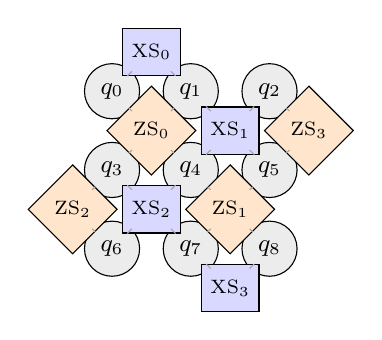
\begin{tikzpicture}[
    data/.style={circle,draw,fill=gray!15,minimum size=7mm,font=\small},
    xanc/.style={rectangle,draw,fill=blue!15,minimum size=6mm,font=\scriptsize},
    zanc/.style={diamond,draw,fill=orange!20,minimum size=7mm,font=\scriptsize},
    link/.style={gray!70,thin}
  ]
  % data qubits q_{3y+x} at (x, 2-y)
  \foreach \x/\y/\lbl in {0/2/0,1/2/1,2/2/2, 0/1/3,1/1/4,2/1/5, 0/0/6,1/0/7,2/0/8}{
    \node[data] (d\lbl) at (\x,\y) {$q_{\lbl}$};
  }
  % X-ancillas
  \node[xanc] (x0) at (0.5,2.5) {XS$_0$};
  \node[xanc] (x1) at (1.5,1.5) {XS$_1$};
  \node[xanc] (x2) at (0.5,0.5) {XS$_2$};
  \node[xanc] (x3) at (1.5,-0.5) {XS$_3$};
  % Z-ancillas
  \node[zanc] (z0) at (0.5,1.5) {ZS$_0$};
  \node[zanc] (z1) at (1.5,0.5) {ZS$_1$};
  \node[zanc] (z2) at (-0.5,0.5) {ZS$_2$};
  \node[zanc] (z3) at (2.5,1.5) {ZS$_3$};
  % links
  \draw[link] (x0)--(d0); \draw[link] (x0)--(d1);
  \draw[link] (x1)--(d1); \draw[link] (x1)--(d2); \draw[link] (x1)--(d4); \draw[link] (x1)--(d5);
  \draw[link] (x2)--(d3); \draw[link] (x2)--(d4); \draw[link] (x2)--(d6); \draw[link] (x2)--(d7);
  \draw[link] (x3)--(d7); \draw[link] (x3)--(d8);
  \draw[link] (z0)--(d0); \draw[link] (z0)--(d1); \draw[link] (z0)--(d3); \draw[link] (z0)--(d4);
  \draw[link] (z1)--(d4); \draw[link] (z1)--(d5); \draw[link] (z1)--(d7); \draw[link] (z1)--(d8);
  \draw[link] (z2)--(d3); \draw[link] (z2)--(d6);
  \draw[link] (z3)--(d2); \draw[link] (z3)--(d5);
\end{tikzpicture}
\caption{Distance-3 rotated surface code layout. Grey circles: data qubits ($q_0$--$q_8$). Blue squares: $X$-type ancillas (detect $Z$ errors, truncated to weight 2 at the top/bottom boundary). Orange diamonds: $Z$-type ancillas (detect $X$ errors, truncated to weight 2 at the left/right boundary). $\bar X$ runs down the left column ($q_0,q_3,q_6$); $\bar Z$ runs across the top row ($q_0,q_1,q_2$).}
\label{fig:lattice}
\end{figure}

\subsection{Independent verification}\label{sec:selftest}

Because the lattice was derived rather than transcribed, it was verified independently of the FPGA circuit implementation using \texttt{qiskit.quantum\_info}, before any hardware was touched. The verification checks, run as a pre-flight self-test ahead of every hardware invocation:
\begin{itemize}
\item every pair of same-type stabilizers commutes (trivially true for same-Pauli-letter operators, checked regardless);
\item every $X$-type stabilizer commutes with every $Z$-type stabilizer (even support overlap);
\item $\bar X$ and $\bar Z$ each commute with all eight stabilizers, and anticommute with each other;
\item the code state obtained by projecting $\lvert 0\rangle^{\otimes 9}$ onto the joint $+1$ eigenspace of the four $X$-stabilizers (via explicit operator projectors $\tfrac12(I+\mathrm{XS}_i)$ applied in sequence) has expectation value $+1$ for every one of the eight stabilizers and for $\bar Z$;
\item every possible single-qubit $Z$ error, and every possible single-qubit $X$ error, decodes (Section~\ref{sec:decoder}) to a correction that leaves the corresponding logical operator's value unchanged.
\end{itemize}
This amounts to 93 independent assertions, all of which pass (Section~\ref{sec:results}). The final class of check -- exhaustive single-qubit-error decoding -- caught a real defect in an early version of the decoding-graph construction, discussed as a case study in Section~\ref{sec:decoder}.

% =============================================================================
\section{Host/FPGA co-execution protocol}\label{sec:protocol}
% =============================================================================

\subsection{Design}

Given the execution model of Section~\ref{sec:background-fpga}, a syndrome round cannot be expressed as "measure the ancillas, branch, reset" within a single kernel invocation. Instead, each round is dispatched to the FPGA as one purely unitary circuit, and the measurement that a real device would perform in hardware is instead performed on the host, by exact Born-rule sampling of the statevector the FPGA kernel returns -- mathematically identical to what a physical device's own classical control system would compute from its measurement record, just executed between kernel launches rather than inside one. Algorithm~\ref{alg:round} summarises one round; Figure~\ref{fig:pipeline} shows the resulting host/FPGA data flow.

\begin{algorithm}
\caption{One syndrome-extraction round (host-orchestrated, FPGA-executed)}\label{alg:round}
\begin{algorithmic}[1]
\Require current 17-qubit statevector $\lvert\psi\rangle$; ancillas that read $1$ last round, $R_{X}, R_{Z}$
\State $G \gets \{\}$
\For{$a \in R_{X}\cup R_{Z}$} \Comment{physically reset last round's ancillas}
    \State $G \gets G \cup \{X(a)\}$
\EndFor
\For{$d \in \text{data qubits}$}
    \State with prob.\ $p$: $G \gets G \cup \{X(d)\}$; with prob.\ $p$: $G \gets G \cup \{Z(d)\}$ \Comment{synthetic error}
\EndFor
\For{each $Z$-stabilizer with support $S$, ancilla $a$}
    \State $G \gets G \cup \{\mathrm{CX}(d,a) : d \in S\}$ \Comment{measure-$Z$, Fig.~1b of~\cite{fowler2012}}
\EndFor
\For{each $X$-stabilizer with support $S$, ancilla $a$}
    \State $G \gets G \cup \{H(a)\} \cup \{\mathrm{CX}(a,d): d\in S\} \cup \{H(a)\}$ \Comment{measure-$X$, Fig.~1c of~\cite{fowler2012}}
\EndFor
\State $\lvert\psi'\rangle \gets \textsc{FpgaRunCircuit}(\lvert\psi\rangle, G)$ \Comment{exact statevector, real hardware}
\State $b \gets \textsc{SampleBornOutcome}(\lvert\psi'\rangle, \text{ancilla qubits})$ \Comment{host, exact Born-rule sampling}
\State $\lvert\psi''\rangle \gets \textsc{ProjectAndRenormalise}(\lvert\psi'\rangle, b)$
\State $R_{X} \gets \{a\in X\text{-ancillas}: b_a=1\}$; $R_{Z} \gets \{a\in Z\text{-ancillas}: b_a=1\}$
\State \Return $\lvert\psi''\rangle$, syndrome bits $b$ (optionally corrupted per Section~\ref{sec:protocol-noise}), $R_X, R_Z$
\end{algorithmic}
\end{algorithm}

The CNOTs within a single stabilizer are scheduled in a simple, deterministic top-to-bottom, left-to-right order. Any ordering of commuting-target CNOTs onto the same ancilla yields an identical final parity, so this ordering is functionally correct; it is not, however, the hook-error-optimal NW/NE/SW/SE schedule of~\cite{tomita2014,fowler2012}, which matters for circuit-level noise injected \emph{during} the entangling gates. Because this study's noise model injects errors between rounds rather than mid-gate (Section~\ref{sec:protocol-noise}), hook-error propagation is not exercised here; adopting the optimal schedule is noted as future work (Section~\ref{sec:discussion}).

\begin{figure}[t]
\centering
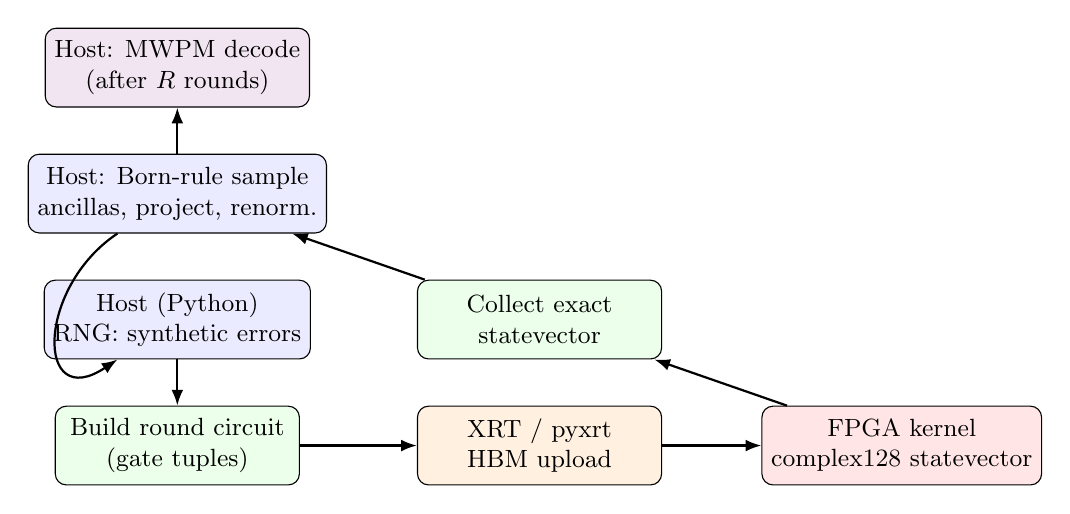
\begin{tikzpicture}[
    box/.style={rectangle,draw,rounded corners,minimum width=3.1cm,minimum height=1.0cm,align=center,font=\small},
    arr/.style={-{Latex[length=2mm]},thick}
  ]
  \node[box,fill=blue!8] (host) at (0,0) {Host (Python)\\RNG: synthetic errors};
  \node[box,fill=green!8] (build) at (0,-1.6) {Build round circuit\\(gate tuples)};
  \node[box,fill=orange!12] (xrt) at (4.6,-1.6) {XRT / pyxrt\\HBM upload};
  \node[box,fill=red!10] (kernel) at (9.2,-1.6) {FPGA kernel\\complex128 statevector};
  \node[box,fill=green!8] (collect) at (4.6,0) {Collect exact\\statevector};
  \node[box,fill=blue!8] (sample) at (0,1.6) {Host: Born-rule sample\\ancillas, project, renorm.};
  \node[box,fill=violet!10] (decode) at (0,3.2) {Host: MWPM decode\\(after $R$ rounds)};

  \draw[arr] (host) -- (build);
  \draw[arr] (build) -- (xrt);
  \draw[arr] (xrt) -- (kernel);
  \draw[arr] (kernel) -- (collect);
  \draw[arr] (collect) -- (sample);
  \draw[arr] (sample) .. controls (-1.8,0.4) and (-1.8,-1.2) .. (host);
  \draw[arr] (sample) -- (decode);
\end{tikzpicture}
\caption{Host/FPGA co-execution loop for one syndrome round. Every entangling operation (error injection, ancilla reset, measure-$Z$/measure-$X$ circuits) runs on the FPGA kernel; only Born-rule sampling, projection, and the classical MWPM decoder run on the host.}
\label{fig:pipeline}
\end{figure}

\subsection{Synthetic syndrome data generation}\label{sec:protocol-noise}

Following~\cite{dennis2002}, three independent error channels share one probability $p$ per round: (i) a bit-flip ($X$) error on each data qubit with probability $p$; (ii) a phase-flip ($Z$) error on each data qubit with probability $p$; and (iii) a bit-flip on each \emph{recorded} syndrome bit with probability $q_{\mathrm{meas}}$ (default $q_{\mathrm{meas}}=p$), applied only to the classical record the decoder sees, never to the physical ancilla state used to drive the next round's reset -- this distinguishes a genuine measurement error (a misread of a correctly prepared ancilla) from a physical qubit error. The final round of each trial is recorded without measurement-bit-flip noise, the standard time-boundary closure that lets a finite-round decoding graph terminate cleanly~\cite{dennis2002,fowler2012}. This construction gives a fully synthetic, reproducible syndrome history -- no physical qubits are involved anywhere in the pipeline -- while remaining a faithful re-implementation of the error model the accuracy-threshold literature analyses.

The experiment tracks a single logical observable per run (by default $\bar Z$, i.e.\ a $\lvert 0\rangle_L$ memory protected against the accumulated $X$-error channel via the $Z$-stabilizer graph); an $\bar X$/$\lvert +\rangle_L$ run is obtained symmetrically by Hadamard-preparing the data register and decoding via the $X$-stabilizer graph instead.

% =============================================================================
\section{Decoding: space-time matching graph}\label{sec:decoder}
% =============================================================================

\subsection{Graph construction}

For each stabilizer type, a space-time graph is built with one node per (stabilizer, round) pair. Spatial edges (weight 1) connect two same-round, same-type stabilizers whose supports share exactly one data qubit -- the qubit that a single physical error on it would flip both eigenvalues of. Temporal edges (weight 1) connect the same stabilizer in consecutive rounds, representing a syndrome \emph{measurement} error rather than a data-qubit error; a matched pair of detection events joined only by temporal edges therefore contributes no physical-qubit correction. Boundary edges connect a stabilizer to one shared virtual boundary node.

The correct, general rule for boundary edges -- and the one this paper's implementation ultimately uses -- is topological rather than based on stabilizer weight: each data qubit belongs to at most two same-type stabilizers by construction (an invariant checked programmatically); a qubit belonging to exactly two is already represented by the spatial edge between them, while a qubit belonging to exactly one has no same-round partner and must connect \emph{directly} to the boundary from its sole owner, regardless of that stabilizer's weight.

\subsection{A decoding-graph pitfall, found by the self-test}

An earlier version of this code restricted boundary edges to weight-2 ("boundary-type") stabilizers only, on the reasoning that those are the ones the lattice derivation of Section~\ref{sec:code} explicitly truncates at a physical edge. This is wrong: two of the four interior, weight-4 stabilizers (XS$_1$ and XS$_2$ in Table~\ref{tab:stabilizers}) each own a data qubit ($q_2,q_5$ and $q_3,q_6$ respectively) that no neighbouring stabilizer shares, because the lattice derivation keeps only one of the two colour-alternating boundary candidates at each physical edge (Section~\ref{sec:code}). Under the restricted rule, a single physical $Z$ error on, e.g., $q_2$ produces a lone detection event at XS$_1$ with no direct boundary edge; the decoder was then forced to route through a neighbour (XS$_0\to$boundary), returning a correction on $\{q_0,q_1\}$ that leaves a residual operator with \emph{odd} overlap with $\bar X$'s support -- a logical error induced by a single weight-1 physical error, which directly violates the distance-3 guarantee that every weight-1 error is uniquely (or at least logically-equivalently) correctable.

This was caught, not by inspection, but by the exhaustive single-qubit-error sweep in the self-test (Section~\ref{sec:selftest}): four of nine single-$Z$-error cases failed their logical-preservation check under the restricted rule. Generalising the boundary rule to the topological (ownership-degree) criterion above -- rather than the weight-based one -- resolved all 93 self-test assertions (Section~\ref{sec:results}). We report this as a general lesson for anyone implementing a matching-graph decoder for a new stabilizer code by hand: boundary connectivity should be derived from qubit-ownership degree in the stabilizer-support graph, not from stabilizer weight, and an exhaustive single-error sweep against an independent (non-graph-based) success criterion is an effective and cheap pre-deployment check.

We note that some qubits remain \emph{syndrome-degenerate} even after this fix -- a single $Z$ error on $q_2$ and a single $Z$ error on $q_5$ produce identical syndromes (both owned solely by XS$_1$) and are therefore indistinguishable to any decoder acting on the syndrome alone. This is expected code degeneracy, not a bug: because neither qubit lies in $\bar X$'s support, either choice of correction leaves the logical value unchanged, and the correct success criterion for a decoded correction is that the true error exclusive-ORed with the correction has even overlap with the relevant logical operator's support -- not that it reproduces the physical error's exact location~\cite{dennis2002}.

\subsection{Matching}

Detection events are collected across all $R$ rounds by XOR-ing each round's recorded syndrome against the previous round's. The matching problem is solved exactly by brute-force enumeration over all perfect matchings of the detection-event set, augmented with one virtual boundary-node copy per event (so every event can independently match "to the boundary"), using precomputed breadth-first-search distances over the unweighted space-time graph. This is exact and fast at the event counts a distance-3 code produces at realistic $p$ (typically 0--6 events per trial); a greedy nearest-neighbour fallback is used above 12 simultaneous events, which never triggered in this study's parameter range. Scaling to larger code distances would require replacing this solver with a library implementation such as PyMatching~\cite{higgott2022} or a Union-Find decoder~\cite{delfosse2021} (Section~\ref{sec:discussion}).

% =============================================================================
\section{Experimental setup}\label{sec:setup}
% =============================================================================

\textbf{Hardware.} A single AMD/Xilinx Alveo U55C accelerator card (shell \texttt{xilinx\_u55c\_gen3x16\_xdma\_base\_3}), hosted in a Gigabyte G292-Z43 server (64 logical CPU cores, 256\,GB RAM, Ubuntu 20.04.6 LTS, kernel 5.4.0), running Xilinx Runtime (XRT) 2.15.225. The kernel was built with Vitis HLS/\texttt{v++} with a 225\,MHz clock target configured in the link stage; the post-route implementation report for this build recorded differing per-domain clocks ($\sim$500\,MHz kernel, $\sim$300\,MHz data, $\sim$450\,MHz HBM AXI), so all timings reported below are measured host-observed wall-clock times, not clock-cycle estimates.

\textbf{Software.} Python 3.8 host driver over \texttt{pyxrt}; NumPy 1.24 for host-side Born-rule sampling and state projection; Qiskit 1.2.4 used only for the independent self-test verification layer of Section~\ref{sec:selftest}, not for circuit execution.

\textbf{Code and protocol.} The distance-3 rotated surface code of Section~\ref{sec:code} (17 of 28 available qubits), logical-$\bar Z$ memory experiment ($\lvert 0\rangle_L$ preparation, decoded against the accumulated $X$-error channel via the $Z$-stabilizer graph). $R=4$ syndrome-extraction rounds per trial; $q_{\mathrm{meas}}=p$ except on the final round (Section~\ref{sec:protocol-noise}); 30 independent trials per physical error rate; $p\in\{0.01,0.03,0.05,0.08,0.12\}$; pseudo-random seed fixed at 1234 for reproducibility.

\textbf{Metric.} Logical error rate: the fraction of trials in which the decoded correction, exclusive-ORed with the true (classically tracked) accumulated error, has odd overlap with $\bar Z$'s support -- i.e.\ the decoder failed to preserve the encoded logical value.

\textbf{Built-in cross-validation.} Because $\bar Z$ commutes with every stabilizer of both types by construction (Section~\ref{sec:code}), its value is provably unperturbed by stabilizer \emph{measurement} and can only change under the accumulated physical $X$-error channel -- meaning it is deterministic given that channel, independent of any stabilizer measurement randomness. Every trial therefore also samples the true final data-qubit register directly from the exact FPGA-returned statevector and compares the resulting logical bit against the independently tracked classical Pauli frame; a mismatch would raise an assertion and abort the run. This ran, silently, on every one of the 150 trials reported below.

% =============================================================================
\section{Results}\label{sec:results}
% =============================================================================

\subsection{Static verification}

All 93 self-test assertions of Section~\ref{sec:selftest} pass: pairwise stabilizer commutation (48 checks), logical-operator commutation with every stabilizer and anticommutation with each other (17 checks), code-state stabilizer/logical eigenvalues (9 checks), and exhaustive single-qubit $Z$- and $X$-error decoding preserving the relevant logical operator (18 checks), plus one two-error independence check.

\subsection{Hardware/software cross-validation}

Across the full sweep (150 trials, 600 FPGA-executed syndrome rounds -- $4$ rounds $\times$ 30 trials $\times$ 5 physical error rates), zero discrepancies were observed between the FPGA-computed statevector's sampled logical readout and the independently tracked classical Pauli frame. This gives empirical, hardware-level confidence that the kernel's numerics, the host-side gate lowering, and the Born-rule sampling/projection implementation are all mutually consistent, in addition to the purely algebraic self-test of Section~\ref{sec:selftest}.

\subsection{Logical error rate versus physical error rate}

\begin{table}[t]
\centering
\caption{Logical error rate versus physical error rate $p$, $R=4$ rounds, 30 trials each, distance-3 rotated surface code on real Alveo U55C hardware. The $p=0.01$ row's upper bound is the exact (Clopper--Pearson) 95\% confidence bound for zero events in 30 trials.}
\label{tab:results}
\begin{tabular}{@{}lllll@{}}
\toprule
$p$ & trials & logical failures & logical error rate & mean wall time/round \\
\midrule
0.01 & 30 & 0  & 0.000 ($\le 0.095$ at 95\% CI) & 353.6\,ms \\
0.03 & 30 & 5  & 0.167 & 358.8\,ms \\
0.05 & 30 & 8  & 0.267 & 369.7\,ms \\
0.08 & 30 & 15 & 0.500 & 375.4\,ms \\
0.12 & 30 & 14 & 0.467 & 389.1\,ms \\
\bottomrule
\end{tabular}
\end{table}

Table~\ref{tab:results} and Figure~\ref{fig:results} summarise the sweep. At $p=1\%$, zero logical failures were observed in 30 trials (exact Clopper--Pearson 95\% upper bound $\approx 9.5\%$); by $p=3\%$ the logical error rate has already risen to 16.7\%, and continues rising (with one non-monotonic point at $p=0.12$, within the sampling noise expected at $n=30$) to roughly 50\% by $p=8$--12\%, where the code offers essentially no protection. The mean wall-clock time per syndrome round rises mildly with $p$ (354\,ms at $p=0.01$ to 389\,ms at $p=0.12$), consistent with the growing number of injected error gates and ancilla-reset gates dispatched per round as the syndrome becomes non-trivial more often; total sweep time was 221.7\,s (excluding the pre-flight self-test) for all 600 rounds.

\begin{figure}[t]
\centering
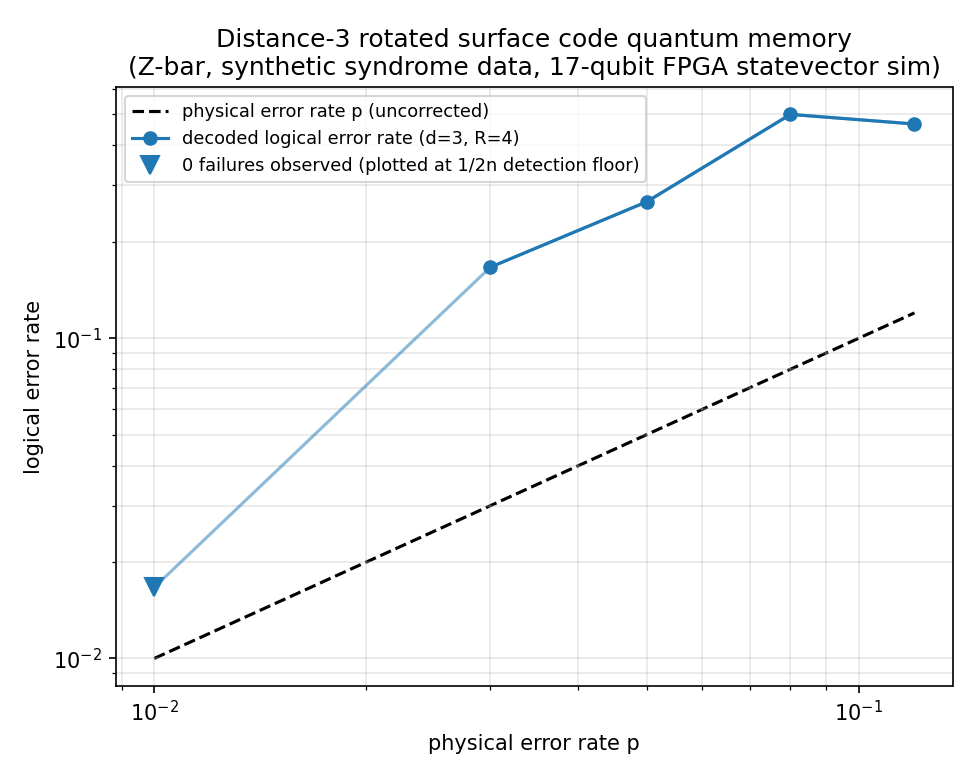
\includegraphics[width=0.85\linewidth]{figures/fig_logical_error_rate.png}
\caption{Decoded logical error rate versus physical error rate $p$ (distance-3, $R=4$ rounds, 30 trials/point, real FPGA hardware). Dashed line: uncorrected physical error rate $p$ for reference. The $p=0.01$ point (triangle marker) is plotted at the $1/2n$ trial-limited detection floor, since zero failures were observed at that point.}
\label{fig:results}
\end{figure}

% =============================================================================
\section{Discussion}\label{sec:discussion}
% =============================================================================

\textbf{Threshold-like behaviour.} The qualitative shape of Table~\ref{tab:results} -- a sharp jump in logical error rate between $p=1\%$ and $p=3\%$ -- is consistent, in order of magnitude, with the $\sim$1.14\% accuracy threshold reported by~\cite{dennis2002}. This should not, however, be over-read as a threshold \emph{measurement}: a genuine threshold determination requires sweeping multiple code distances and locating the $p$ at which the logical-error-rate curves for different $d$ cross~\cite{fowler2012,acharya2023}, whereas this study reports a single distance ($d=3$) at a single round count ($R=4$) with a modest sample size (30 trials/point, giving wide confidence intervals particularly at the zero-failure point). The result presented here should be read as a qualitative, hardware-validated consistency check against the literature, not a threshold estimate.

\textbf{Why the logical rate exceeds $p$ so quickly.} With $q_{\mathrm{meas}}=p$ applied to eight ancilla readouts across three (of four) rounds, plus independent $X$/$Z$ channels on nine data qubits across all four rounds, the effective per-trial error budget is substantially larger than the bare per-qubit $p$ -- by design, since this mirrors~\cite{dennis2002}'s model rather than a single-shot error rate. This explains why the logical error rate climbs above $p$ so much faster than a naive single-round picture would suggest.

\textbf{Scope limitations.} (i) The CNOT scheduling within each stabilizer (Section~\ref{sec:protocol}) is a simple deterministic ordering, not the hook-error-optimal schedule of~\cite{tomita2014}; since this study's noise model does not inject errors during the entangling gates themselves, this does not affect the results reported here but would need addressing before extending the noise model to circuit-level (gate-time) errors. (ii) The brute-force matching decoder (Section~\ref{sec:decoder}) does not scale past the small event counts a distance-3 code produces; adopting PyMatching~\cite{higgott2022} or a Union-Find decoder~\cite{delfosse2021} is necessary for larger distances. (iii) Only a single logical qubit and a single code distance were studied. (iv) The error model uses independent $X$/$Z$ channels rather than a full depolarizing or leakage model. (v) Most importantly for an embedded-systems readership: the $\sim$350--390\,ms measured wall time per syndrome round is dominated by host$\leftrightarrow$FPGA HBM transfer of the 17-qubit ($2^{17}$-amplitude) statevector and kernel-launch overhead for what is a numerically tiny circuit -- several orders of magnitude slower than the sub-microsecond syndrome-to-correction latency targeted by dedicated real-time decoder pipelines such as our companion work~\cite{ali_shor_steane_qec}. This is expected and, for the purposes of this paper, acceptable: the goal here is exact-state \emph{algorithmic correctness validation} of the full surface-code protocol, not real-time decoding throughput. The two goals are complementary: an exact-statevector validation harness of the kind reported here gives a verifiable ground truth that a fast, approximate, hardware-streamed decoder pipeline can be benchmarked against.

\textbf{Value of the host/FPGA co-execution pattern.} Beyond the specific surface-code result, Section~\ref{sec:protocol}'s protocol -- dispatch one purely unitary circuit per round, perform only the unavoidable measurement collapse and classical decoding on the host, and feed the collapsed state forward via explicit state reload -- is a general pattern for validating any repeated-measurement fault-tolerance protocol on accelerator hardware that lacks native mid-circuit classical feedback, which describes a meaningful fraction of currently deployed FPGA/GPU statevector kernels, including prior systems in this same hardware family~\cite{ali_rtl_statevector,ali_30qubit_sim}.

% =============================================================================
\section{Conclusion and future work}\label{sec:conclusion}
% =============================================================================

This paper implemented a distance-3 rotated surface code, derived and independently verified from first principles, on a 28-qubit HBM-accelerated FPGA statevector simulator, and demonstrated a host/FPGA co-execution protocol for running a genuine multi-round fault-tolerant quantum-memory experiment on hardware that offers no native mid-circuit measurement-and-branch instruction -- every entangling operation still executes on the FPGA kernel, and only the physically unavoidable measurement collapse and classical MWPM decoding run on the host. A synthetic-syndrome-data generator reproduced the Dennis--Kitaev--Landahl--Preskill error model, and a from-scratch space-time matching decoder -- whose construction is reported together with a real connectivity bug we found and fixed via exhaustive self-testing -- decoded 150 hardware trials (600 FPGA-executed syndrome rounds) with zero discrepancies against an independent classical cross-check, producing a logical-error-rate curve qualitatively consistent with the literature's reported accuracy threshold.

Future work includes: (i) scaling within the 28-qubit budget to larger code patches or a second logical qubit; (ii) adding a native mid-circuit ancilla measurement-and-reset primitive to the kernel itself, removing the host round-trip that currently dominates wall time; (iii) replacing the brute-force matching solver with PyMatching or a Union-Find decoder to support larger code distances; (iv) extending the noise model to full depolarizing and leakage channels; (v) cross-validating against Stim at the stabilizer-circuit level; (vi) extending to logical two-qubit operations via lattice surgery; and (vii) coupling this exact-state validation harness to the real-time FPGA decoder pipeline of~\cite{ali_shor_steane_qec} for an end-to-end demonstration that combines exact-state correctness validation with real-time decoding latency on the same hardware family.

% =============================================================================
\backmatter

\section*{Declarations}

\textbf{Funding.} This work was carried out at the Centre for Development of Advanced Computing (C-DAC), Noida, India. \emph{[Author: insert specific grant/project number, if applicable, before submission.]}

\textbf{Conflict of interest.} The author declares no conflict of interest.

\textbf{Data and code availability.} The FPGA host driver, surface-code circuit generator, decoder implementation, and the result data (CSV) and figure reported in Section~\ref{sec:results} are available from the corresponding author upon reasonable request, and may be published in a public repository (e.g.\ \url{https://github.com/nasir26}) prior to final submission. \emph{[Author: confirm final hosting location/DOI before submission.]}

\textbf{Author contribution.} N.A.\ conceived the study, derived and verified the surface-code lattice and decoder, implemented the host/FPGA co-execution protocol, ran the hardware experiments, and wrote the manuscript.

% =============================================================================
\begin{thebibliography}{99}

\bibitem{kitaev2003} Kitaev, A.Y.: Fault-tolerant quantum computation by anyons. Ann. Phys. \textbf{303}(1), 2--30 (2003)

\bibitem{bravyikitaev1998} Bravyi, S.B., Kitaev, A.Y.: Quantum codes on a lattice with boundary. arXiv:quant-ph/9811052 (1998)

\bibitem{dennis2002} Dennis, E., Kitaev, A., Landahl, A., Preskill, J.: Topological quantum memory. J. Math. Phys. \textbf{43}(9), 4452--4505 (2002)

\bibitem{fowler2012} Fowler, A.G., Mariantoni, M., Martinis, J.M., Cleland, A.N.: Surface codes: Towards practical large-scale quantum computation. Phys. Rev. A \textbf{86}, 032324 (2012)

\bibitem{tomita2014} Tomita, Y., Svore, K.M.: Low-distance surface codes under realistic quantum noise. Phys. Rev. A \textbf{90}, 062320 (2014)

\bibitem{versluis2017} Versluis, R., Poletto, S., Khammassi, N., Tarasinski, B., Haider, N., Michalak, D.J., Bruno, A., Bertels, K., DiCarlo, L.: Scalable quantum circuit and control for a superconducting surface code. Phys. Rev. Appl. \textbf{8}, 034021 (2017)

\bibitem{acharya2023} Google Quantum AI (Acharya, R., et al.): Suppressing quantum errors by scaling a surface code logical qubit. Nature \textbf{614}, 676--681 (2023)

\bibitem{chamberland2020} Chamberland, C., Zhu, G., Yoder, T.J., Hertzberg, J.B., Cross, A.W.: Topological and subsystem codes on low-degree graphs with flag qubits. Phys. Rev. X \textbf{10}, 011022 (2020)

\bibitem{edmonds1965} Edmonds, J.: Paths, trees, and flowers. Canad. J. Math. \textbf{17}, 449--467 (1965)

\bibitem{higgott2022} Higgott, O.: PyMatching: A Python package for decoding quantum codes with minimum-weight perfect matching. ACM Trans. Quantum Comput. \textbf{3}(3), 1--16 (2022) \% VERIFY exact page range before submission.

\bibitem{delfosse2021} Delfosse, N., Nickerson, N.H.: Almost-linear time decoding algorithm for topological codes. Quantum \textbf{5}, 595 (2021)

\bibitem{gidney2021stim} Gidney, C.: Stim: a fast stabilizer circuit simulator. Quantum \textbf{5}, 497 (2021)

\bibitem{qiskit} Javadi-Abhari, A., Treinish, M., Krsulich, K., et al.: Quantum computing with Qiskit. arXiv:2405.08810 (2024)

\bibitem{alveo_u55c} AMD/Xilinx: Alveo U55C High-Performance Compute Card Data Sheet, DS978. AMD/Xilinx, Inc. (2023) \% VERIFY current document number before submission.

\bibitem{vitis_hls} AMD/Xilinx: Vitis Unified Software Platform Documentation: Application Acceleration Development, UG1393. AMD/Xilinx, Inc. \% VERIFY current document number before submission.

\bibitem{xrt} AMD/Xilinx: Xilinx Runtime (XRT) Documentation. \url{https://github.com/Xilinx/XRT}

\bibitem{ali_rtl_statevector} Ali, N.: A Native RTL Quantum Statevector Simulator in FP64 on an HBM-Equipped FPGA. Submitted to J. Supercomput. (2026)

\bibitem{ali_30qubit_sim} Ali, N.: FPGA Based Quantum Circuit Simulator: Processing 30 Qubit Systems. Submitted to J. Supercomput. (2026)

\bibitem{ali_mps_engine} Ali, N.: Matrix Product State Engine for FPGA Quantum Circuit Simulation Beyond Five Hundred Qubits. Submitted to J. Supercomput. (2026)

\bibitem{ali_shor_steane_qec} Ali, N.: FPGA-Based Real-Time Quantum Error Correction for Shor and Steane Codes. Submitted to J. Supercomput. (2026)

\end{thebibliography}

\end{document}
